\documentclass{scrartcl}

\usepackage[british]{babel}
\usepackage{amsfonts}
\usepackage{mathtools}
\usepackage{graphicx}
\usepackage{amsthm}
\usepackage{minted}
\usepackage{algpseudocodex}
\usepackage{booktabs}
\usepackage[pdftitle={Five ways to view matrix-matrix multiplication}, pdfauthor={Noah Tarr}]{hyperref}

\title{Five ways to view matrix-matrix multiplication}
\author{Noah Tarr}
\date{}

\begin{document}
\maketitle

\section{In terms of dimensions}
The product of an \(m \times n\) matrix \(A\) and an \(n \times p\) matrix \(B\) is an \(m \times p\) matrix \(C\).

\section{As composition of linear transformations}
Let \(A\) be an \(m \times n\) matrix.\\
Let \(T_A : \mathbb{R}^n \to \mathbb{R}^m\) be the linear transformation such that \(T_A(\mathbf{x}) = A\mathbf{x}\), where \(A\mathbf{x}\) is matrix-vector multiplication.\\
Let \(B\) be an \(n \times p\) matrix.\\
Let \(T_B : \mathbb{R}^p \to \mathbb{R}^n \) be the linear transformation such that \(T_B(\mathbf{y}) = B\mathbf{y}\).\\
Then \((T_A \circ T_B)(\mathbf{x}) = T_A(T_B(\mathbf{x})) = T_A(B\mathbf{x}) = AB\mathbf{x}\), where \(AB\) is matrix-matrix multiplication.

\section{In terms of other multiplication}
Multiplication of a matrix by a matrix can be seen from five different perspectives:

\begin{itemize}
\item row by column multiplication
\item one column at a time
\item one row at a time
\item as a sum of outer products
\item block multiplication
\end{itemize}

All of them are mathematically equivalent and lead to the same result.

\subsection{Rows by columns}
This is standard matrix multiplication using dot products.\\
For each row of matrix \(A\), calculate a dot product with each column of matrix \(B\).\\
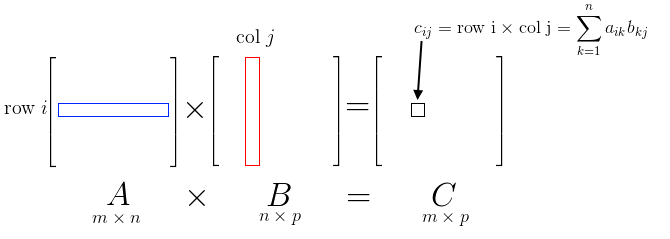
\includegraphics[height=12em]{row-by-columns.png}\\
The \(i\)th component of the \(j\)th column of \(C\) is
\begin{align*}
  c_{ij} &= (\text{row \(i\) of \(A\)})^T \cdot (\text{column \(j\) of \(B\)})\\
         &= (\text{column \(i\) of \(A^T\)}) \cdot (\text{column \(j\) of \(B\)})\\
         &= \mathbf{a}^T_i \cdot \mathbf{b}_j\\
         &= \sum_{k=1}^n{c_{ik}b_{kj}}\text{.}
\end{align*}

\subsection{One column at a time}
A transformation \(T_B\) represented by a matrix \(B\) maps the \(i\)th basis vector to \(\mathbf{b}_i\).\\
A transformation \(T_A\) represented by a matrix \(A\) maps a vector \(\mathbf{x}\) to \(A\mathbf{x}\).\\
Thus, the transformation \(T_A \circ T_B\) maps the \(i\)th basis vector to \(A\mathbf{b}_i\).\\
Let \(C = AB\).\\
Then \(T_A \circ T_B\) is represented by the matrix \(C\).\\
Thus, \(\mathbf{c}_i = A\mathbf{b}_i\).\\
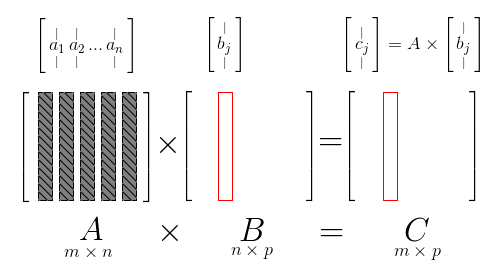
\includegraphics[height=15em]{one-column-at-a-time.png}

\subsection{One row at a time}
The \(i\)th component of \(A\mathbf{x}\) is \(\mathbf{a}^T_i \cdot \mathbf{x} = (\mathbf{a}^T_i)^T\mathbf{x}\).\\
Thus, the \(i\)th component of \(AB\mathbf{y}\) is \((\mathbf{a}^T_i)^TB\mathbf{y}\).\\
Let \(C = AB\).\\
Then
\begin{align*}
  (\mathbf{c}^T_i)^T\mathbf{y} &= (\mathbf{a}^T_i)^TB\mathbf{y}\\
  \implies (\mathbf{c}^T_i)^T &= (\mathbf{a}^T_i)^TB\text{.}
\end{align*}
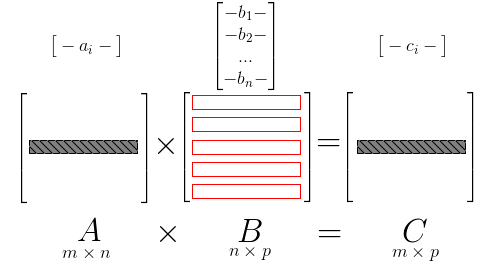
\includegraphics[height=15em]{one-row-at-a-time.png}

\subsection{As a sum of outer products}
\subsubsection*{Algorithm}
Let \(A\) be an \(m \times n\) matrix and \(B\) be an \(n \times p\) matrix.\\
For every \(i \in \mathbb{N}\) from 1 to \(n\), calculate the outer product of \(\mathbf{a}_i\) and \(\mathbf{b}^T_i\).\\
Sum over all these outer products.
\subsubsection*{Formula}
Let \(C = AB\).\\
Then
\begin{align*}
  C &= \sum_{i = 1}^n\mathbf{a}_i \otimes \mathbf{b}^T_i\\
    &= \sum_{i = 1}^n\mathbf{a}_i(\mathbf{b}^T_i)^T\text{.}
\end{align*}
\subsubsection*{Picture}
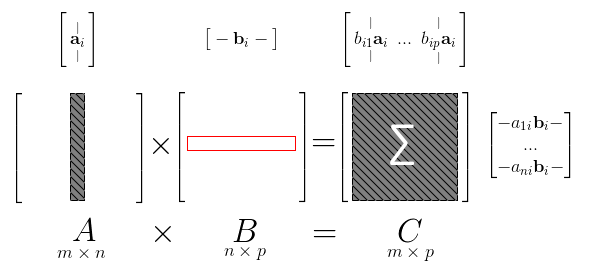
\includegraphics[height=15em]{sum-of-outer-products.png}

\section{As block multiplication}
In the following equation, the variables are rectangular matrices concatenated into one large matrix.
\begin{equation*}
  \begin{bmatrix}
    A_1 & B_1 \\
    C_1 & D_1
  \end{bmatrix}
  \begin{bmatrix}
    A_2 & B_2 \\
    C_2 & D_2
  \end{bmatrix}
  =
  \begin{bmatrix}
    A_1A_2+B_1C_2 & A_1B_2+B_1D_2 \\
    C_1A_2+D_1C_2 & C_1B_2+D_1D_2
  \end{bmatrix}
\end{equation*}

\section{In terms of its properties}
\subsection{Transposition}
\begin{align*}
  (AB)^T &= B^TA^T\\
  (A_1 \dotsm A_n)^T &= A_n^T \dotsm A_1^T
\end{align*}

\subsection{Inverse matrices}
\begin{equation*}
  (AB)^{-1} = B^{-1}A^{-1}
\end{equation*}

\subsubsection*{Algebraic proof}
\begin{align*}
  (AB)(B^{-1}A^{-1}) &= A(BB^{-1})A^{-1}\\
                     &= AIA^{-1}\\
                     &= AA^{-1}\\
                     &= I\\
  (B^{-1}A^{-1})(AB) &= B^{-1}(A^{-1}A)B\\
                     &= B^{-1}IB\\
                     &= B^{-1}B\\
                     &= I
\end{align*}

\subsection{Row space and column space}
Let \(C(A)\) denote the column space of \(A\) and \(R(A)\) denote the row space of \(A\).

\begin{proof}[Proof that \(C(AB) \subseteq C(A)\)]
  Let \(A\) be an \(m \times n\) matrix and \(B\) be an \(n \times p\) matrix.\\
  Let \(T_A(\mathbf{x})\ = A\mathbf{x}\) and \(T_B(\mathbf{x}) = B\mathbf{x}\).\\
  Note that \(\operatorname{image}(T_A \circ T_B) = C(AB)\) and \(\operatorname{image}(T_A) = C(A)\).\\
  Thus, \(C(AB) \subseteq C(A) \impliedby \operatorname{image}(T_A \circ T_B) \subseteq \operatorname{image}(T_A)\), which is shown by the following diagram, in which \(\operatorname{image}(T_A)\) and \(\operatorname{image}(T_A \circ T_B)\) should be swapped.\\
  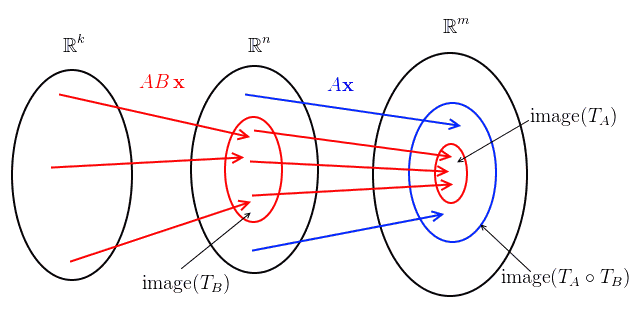
\includegraphics[height=15em]{column-space.png}
\end{proof}

\begin{proof}[Proof that \(R(AB) \subseteq R(B)\)]
  \[R(AB) = C(B^TA^T) \subseteq C(B^T) = R(B)\]
\end{proof}

\section{In terms of its implementation}
\subsection*{In an imperative language}
The following C program executes \(C \gets AB + C\), where \(A\) is an \(m \times r\) matrix, \(B\) is an \(r \times n\) matrix and \(C\) is an \(m \times n\) matrix.
The arrays \mintinline{c}{a}, \mintinline{c}{b} and \mintinline{c}{c} represent \(A\), \(B\) and \(C\), respectively, in row-major order.

\begin{minted}{c}
for (int i = 0; i < m; i++) {
    for (int j = 0; j < n; j++) {
        for (int k = 0; k < r; k++) {
            c[i][j] += a[i][k] * b[k][j];
        }
    }
}
\end{minted}

The \mintinline{c}{i}, \mintinline{c}{j} and \mintinline{c}{k} loops can be rearranged to get the same result from a different algorithm.

\begin{table}[h]
  \centering
  \begin{tabular}{l l l l}
    \toprule
    Order & Inner loop & Middle loop & Inner loop access \\
    \midrule
    \mintinline{c}{i}\mintinline{c}{j}\mintinline{c}{k} & \(c_{ij} \gets (\mathbf{a}^T_i)^T\mathbf{b}_j + c_{ij}\) & \((\mathbf{c}^T_i)^T \gets (\mathbf{a}^T_i)^TB + (\mathbf{c}^T_i)^T\) & \(A\) row, \(B\) column \\
    \mintinline{c}{j}\mintinline{c}{i}\mintinline{c}{k} & \(c_{ij} \gets (\mathbf{a}^T_i)^T\mathbf{b}_j + c_{ij}\) & \(\mathbf{c}_j \gets A\mathbf{b}_j + \mathbf{c}_j\) & \(A\) row, \(B\) column \\
    \mintinline{c}{i}\mintinline{c}{k}\mintinline{c}{j} & \((\mathbf{c}^T_{i})^T \gets (a_{ik}(\mathbf{b}^T_{k})^T + \mathbf{c}^T_{i})^T\) & \((\mathbf{c}^T_i)^T \gets (\mathbf{a}^T_i)^TB + (\mathbf{c}^T_i)^T\) & \(B\) row, \(C\) row \\
    \mintinline{c}{j}\mintinline{c}{k}\mintinline{c}{i} & \(\mathbf{c}_j \gets b_{kj}\mathbf{a}_k + \mathbf{c}_j\) & \(\mathbf{c}_j \gets A\mathbf{b}_j + \mathbf{c}_j\) & \(A\) column, \(B\) column \\
    \mintinline{c}{k}\mintinline{c}{i}\mintinline{c}{j} & \((\mathbf{c}^T_{i})^T \gets a_{ik}(\mathbf{b}^T_{k})^T + (\mathbf{c}^T_{i})^T\) & \(C \gets \mathbf{a}_k(\mathbf{b}^T_{k})^T + C\) & \(A\) row, \(C\) row \\ 
    \mintinline{c}{k}\mintinline{c}{j}\mintinline{c}{i} & \(\mathbf{c}_j \gets b_{kj}\mathbf{a}_k + \mathbf{c}_j\)  & \(C \gets \mathbf{a}_k(\mathbf{b}^T_{k})^T + C\) & \(A\) column, \(C\) column \\
    \bottomrule
  \end{tabular}
\end{table}

The way the inner loop accesses the data determines the most time-efficient way to store the data --- data should be contiguous in memory.

\par
The operation \(\mathbf{y} \gets a\mathbf{x} + \mathbf{y}\) is known as \texttt{saxpy} (scalar \(a\) times \(\mathbf{x}\) plus \(\mathbf{y}\)).
Similarly, \(\mathbf{y} \gets A\mathbf{x} + \mathbf{y}\) is known as \texttt{gaxpy} (generalised \texttt{axpy}).
These are from the Basic Linear Algebra Subprograms specification.

\par
\(A \gets \mathbf{x}\mathbf{y}^T + A\) is called an outer product update.

\iffalse
Each permutation is given in pseudocode is shown below in decreasing levels of abstraction.

\subsubsection*{\mintinline{c}{i}, \mintinline{c}{j}, \mintinline{c}{k}}
\begin{algorithmic}
  \For{\(i = 0, \dotsc, m-1\)}
  \State \((\mathbf{c}^T_i)^T \gets (\mathbf{c}^T_i)^T + (\mathbf{a}^T_i)^TB\)
  \EndFor
\end{algorithmic}
\begin{algorithmic}
  \For{\(i = 0, \dotsc, m-1\)}
  \For{\(j = 0, \dotsc, n-1\)}
  \State \(c_{ij} \gets c_{ij} + (\mathbf{a}^T_i)^T\mathbf{b}_j\)
  \EndFor
  \EndFor
\end{algorithmic}
\begin{algorithmic}
  \For{\(i = 0, \dotsc, m-1\)}
  \For{\(j = 0, \dotsc, n-1\)}
  \For{\(k = 0, \dotsc, r-1\)}
  \State \(c_{ij} \gets c_{ij} + a_{ik}b_{kj}\)
  \EndFor
  \EndFor
  \EndFor
\end{algorithmic}

\subsubsection*{\mintinline{c}{j}, \mintinline{c}{i}, \mintinline{c}{k}}
\begin{algorithmic}
  \For{\(j = 0, \dotsc, m-1\)}
  \State \(\mathbf{c}_j \gets \mathbf{c}_j + A\mathbf{b}_j\)
  \EndFor
\end{algorithmic}
\begin{algorithmic}
  \For{\(j = 0, \dotsc, m-1\)}
  \For{\(i = 0, \dotsc, n-1\)}
  \State \(c_{ij} \gets c_{ij} + (\mathbf{a}^T_i)^T\mathbf{b}_j\)
  \EndFor
  \EndFor
\end{algorithmic}
\begin{algorithmic}
  \For{\(j = 0, \dotsc, m-1\)}
  \For{\(i = 0, \dotsc, n-1\)}
  \For{\(k = 0, \dotsc, r-1\)}
  \State \(c_{ij} \gets c_{ij} + a_{ik}b_{kj}\)
  \EndFor
  \EndFor
  \EndFor
\end{algorithmic}

\subsubsection*{\mintinline{c}{i}, \mintinline{c}{k}, \mintinline{c}{j}}
\begin{algorithmic}
  \For{\(i = 0, \dotsc, m-1\)}
  \State \((\mathbf{c}^T_i)^T \gets (\mathbf{c}^T_i)^T + (\mathbf{a}^T_i)^TB\)
  \EndFor
\end{algorithmic}
\begin{algorithmic}
  \For{\(i = 0, \dotsc, m-1\)}
  \For{\(k = 0, \dotsc, n-1\)}
  \State \((\mathbf{c}^T_{i})^T \gets (\mathbf{c}^T_{i})^T + a_{ik}(\mathbf{b}^T_{k})^T\)
  \EndFor
  \EndFor
\end{algorithmic}
\begin{algorithmic}
  \For{\(i = 0, \dotsc, m-1\)}
  \For{\(k = 0, \dotsc, n-1\)}
  \For{\(j = 0, \dotsc, r-1\)}
  \State \(c_{ij} \gets c_{ij} + a_{ik}b_{kj}\)
  \EndFor
  \EndFor
  \EndFor
\end{algorithmic}

\subsubsection*{\mintinline{c}{j}, \mintinline{c}{k}, \mintinline{c}{i}}
\begin{algorithmic}
  \For{\(j = 0, \dotsc, m-1\)}
  \State \(\mathbf{c}_j \gets \mathbf{c}_j + A\mathbf{b}_j\)
  \EndFor
\end{algorithmic}
\begin{algorithmic}
  \For{\(j = 0, \dotsc, m-1\)}
  \For{\(k = 0, \dotsc, n-1\)}
  \State \(\mathbf{c}_j \gets \mathbf{c}_j + b_{kj}\mathbf{a}_k\)
  \EndFor
  \EndFor
\end{algorithmic}
\begin{algorithmic}
  \For{\(j = 0, \dotsc, m-1\)}
  \For{\(k = 0, \dotsc, n-1\)}
  \For{\(i = 0, \dotsc, r-1\)}
  \State \(c_{ij} \gets c_{ij} + a_{ik}b_{kj}\)
  \EndFor
  \EndFor
  \EndFor
\end{algorithmic}

\subsubsection*{\mintinline{c}{k}, \mintinline{c}{i}, \mintinline{c}{j}}
\begin{algorithmic}
  \For{\(i = 0, \dotsc, m-1\)}
  \For{\(k = 0, \dotsc, n-1\)}
  \State \((\mathbf{c}^T_{i})^T \gets (\mathbf{c}^T_{i})^T + a_{ik}(\mathbf{b}^T_{k})^T\)
  \EndFor
  \EndFor
\end{algorithmic}
\begin{algorithmic}
  \For{\(k = 0, \dotsc, m-1\)}
  \For{\(i = 0, \dotsc, n-1\)}
  \For{\(j = 0, \dotsc, r-1\)}
  \State \(c_{ij} \gets c_{ij} + a_{ik}b_{kj}\)
  \EndFor
  \EndFor
  \EndFor
\end{algorithmic}
\fi

\subsection*{In SQL}
Let \(A\) and \(B\) be matrices stored as tables of \texttt{(row\_num, col\_num, value)} triples.
Then an implementation in SQL follows.
\begin{minted}{sql}
select a.row_num, b.col_num, sum(a.value * b.value)
from A a, B b
where a.col_num = b.row_num
group by a.row_num, b.col_num;
\end{minted}

\subsection*{In MapReduce, using Apache Flink}
The following Java expression executes the same algorithm as the above SQL query, I think.
\begin{minted}{java}
matrixA.join(matrixB).where(1).equalTo(0)
       .map(new ProjectJoinResultMapper()).groupBy(0, 1).sum(2)
\end{minted}

\end{document}
